\section{Extensions}

We will now explore the potential application of the one-step ahead predictor formula with the Kalman Filter in various contexts beyond its original domain.

\subsection{Multi-step prediction}
Assuming that $\hat{x}(t+1|t)$ is known, the $k$-step ahead prediction can be straightforwardly computed. 
Given $\hat{x}(t+1|t)$, we can derive:
\[\begin{cases}
    \hat{x}(t+k|t)=F^{k+1} \hat{x}(t+1|t) \\
    \hat{y}(t+k|t)=H \hat{x}(t+k|t)
\end{cases}\]

\subsection{Filtering}
The filtering process, denoted as $\hat{x}(t|t)$, aims to estimate the current state of the system given available measurements up to time $t$. 
Assuming that $\hat{x}(t+1|t)$ is known, we can compute $\hat{x}(t|t)$ using different formulations based on the properties of the system matrix.

\paragraph*{Straightforward solution}
If the matrix $F$ is invertible, we have a straightforward solution:
\[\hat{x}(t|t)=F^{-1} \hat{x}(t+1|t)\]

\paragraph*{Filter formulation}
In special cases where $F$ is not invertible, we use the filter formulation of the Kalman Filter:
\[\begin{cases}
    \hat{x}(t|t)=F\hat{x}(t-1|t-1)+K_0(t)e(t) \\
    \hat{y}(t|t-1)=H\hat{x}(t|t-1) \\
    e(t)=y(t)-\hat{y(t|t-1)} \\
    K_0(t)=\left(P(t)H^T\right)\left(HP(t)H^T+V_2\right)^{-1} \\
    P(t+1)=\left(FP(T)F^T+V_1\right)-\left(FP(t)H^T+V_{12}\right)\left(HP(t)H^T+V_{2}\right)^{-1}\left(FP(t)H^T+V_{12}\right)^T
\end{cases}\]
The initial condition for the filter is $\hat{x}(1|1)=x_0$. 
The equation for $K_0(t)$ is referred to as the filter gain.
This formula is valid only when $V_{12}=0$, which is typically true in practice.

\paragraph*{Gains}
There's a distinction between two gains when $V_{12}=0$: 
\begin{itemize}
    \item Prediction gain: $K(t)=\left(FP(t)H^T+V_{12}\right)\left(FP(t)H^T+V_2\right)^{-1}$.
    \item Filter gain: $K_0(t)=\left(P(t)H^T\right)\left(HP(t)H^T+V_2\right)^{-1}$.
\end{itemize}
The primary difference lies in the initial $F$, which is absent in the filter gain equation.

\subsection{Exogenous input}
Graphically, the Kalman Filtering process with an eXogenous input $Gu(t)$ is illustrated as follows:
\begin{figure}[H]
    \centering
    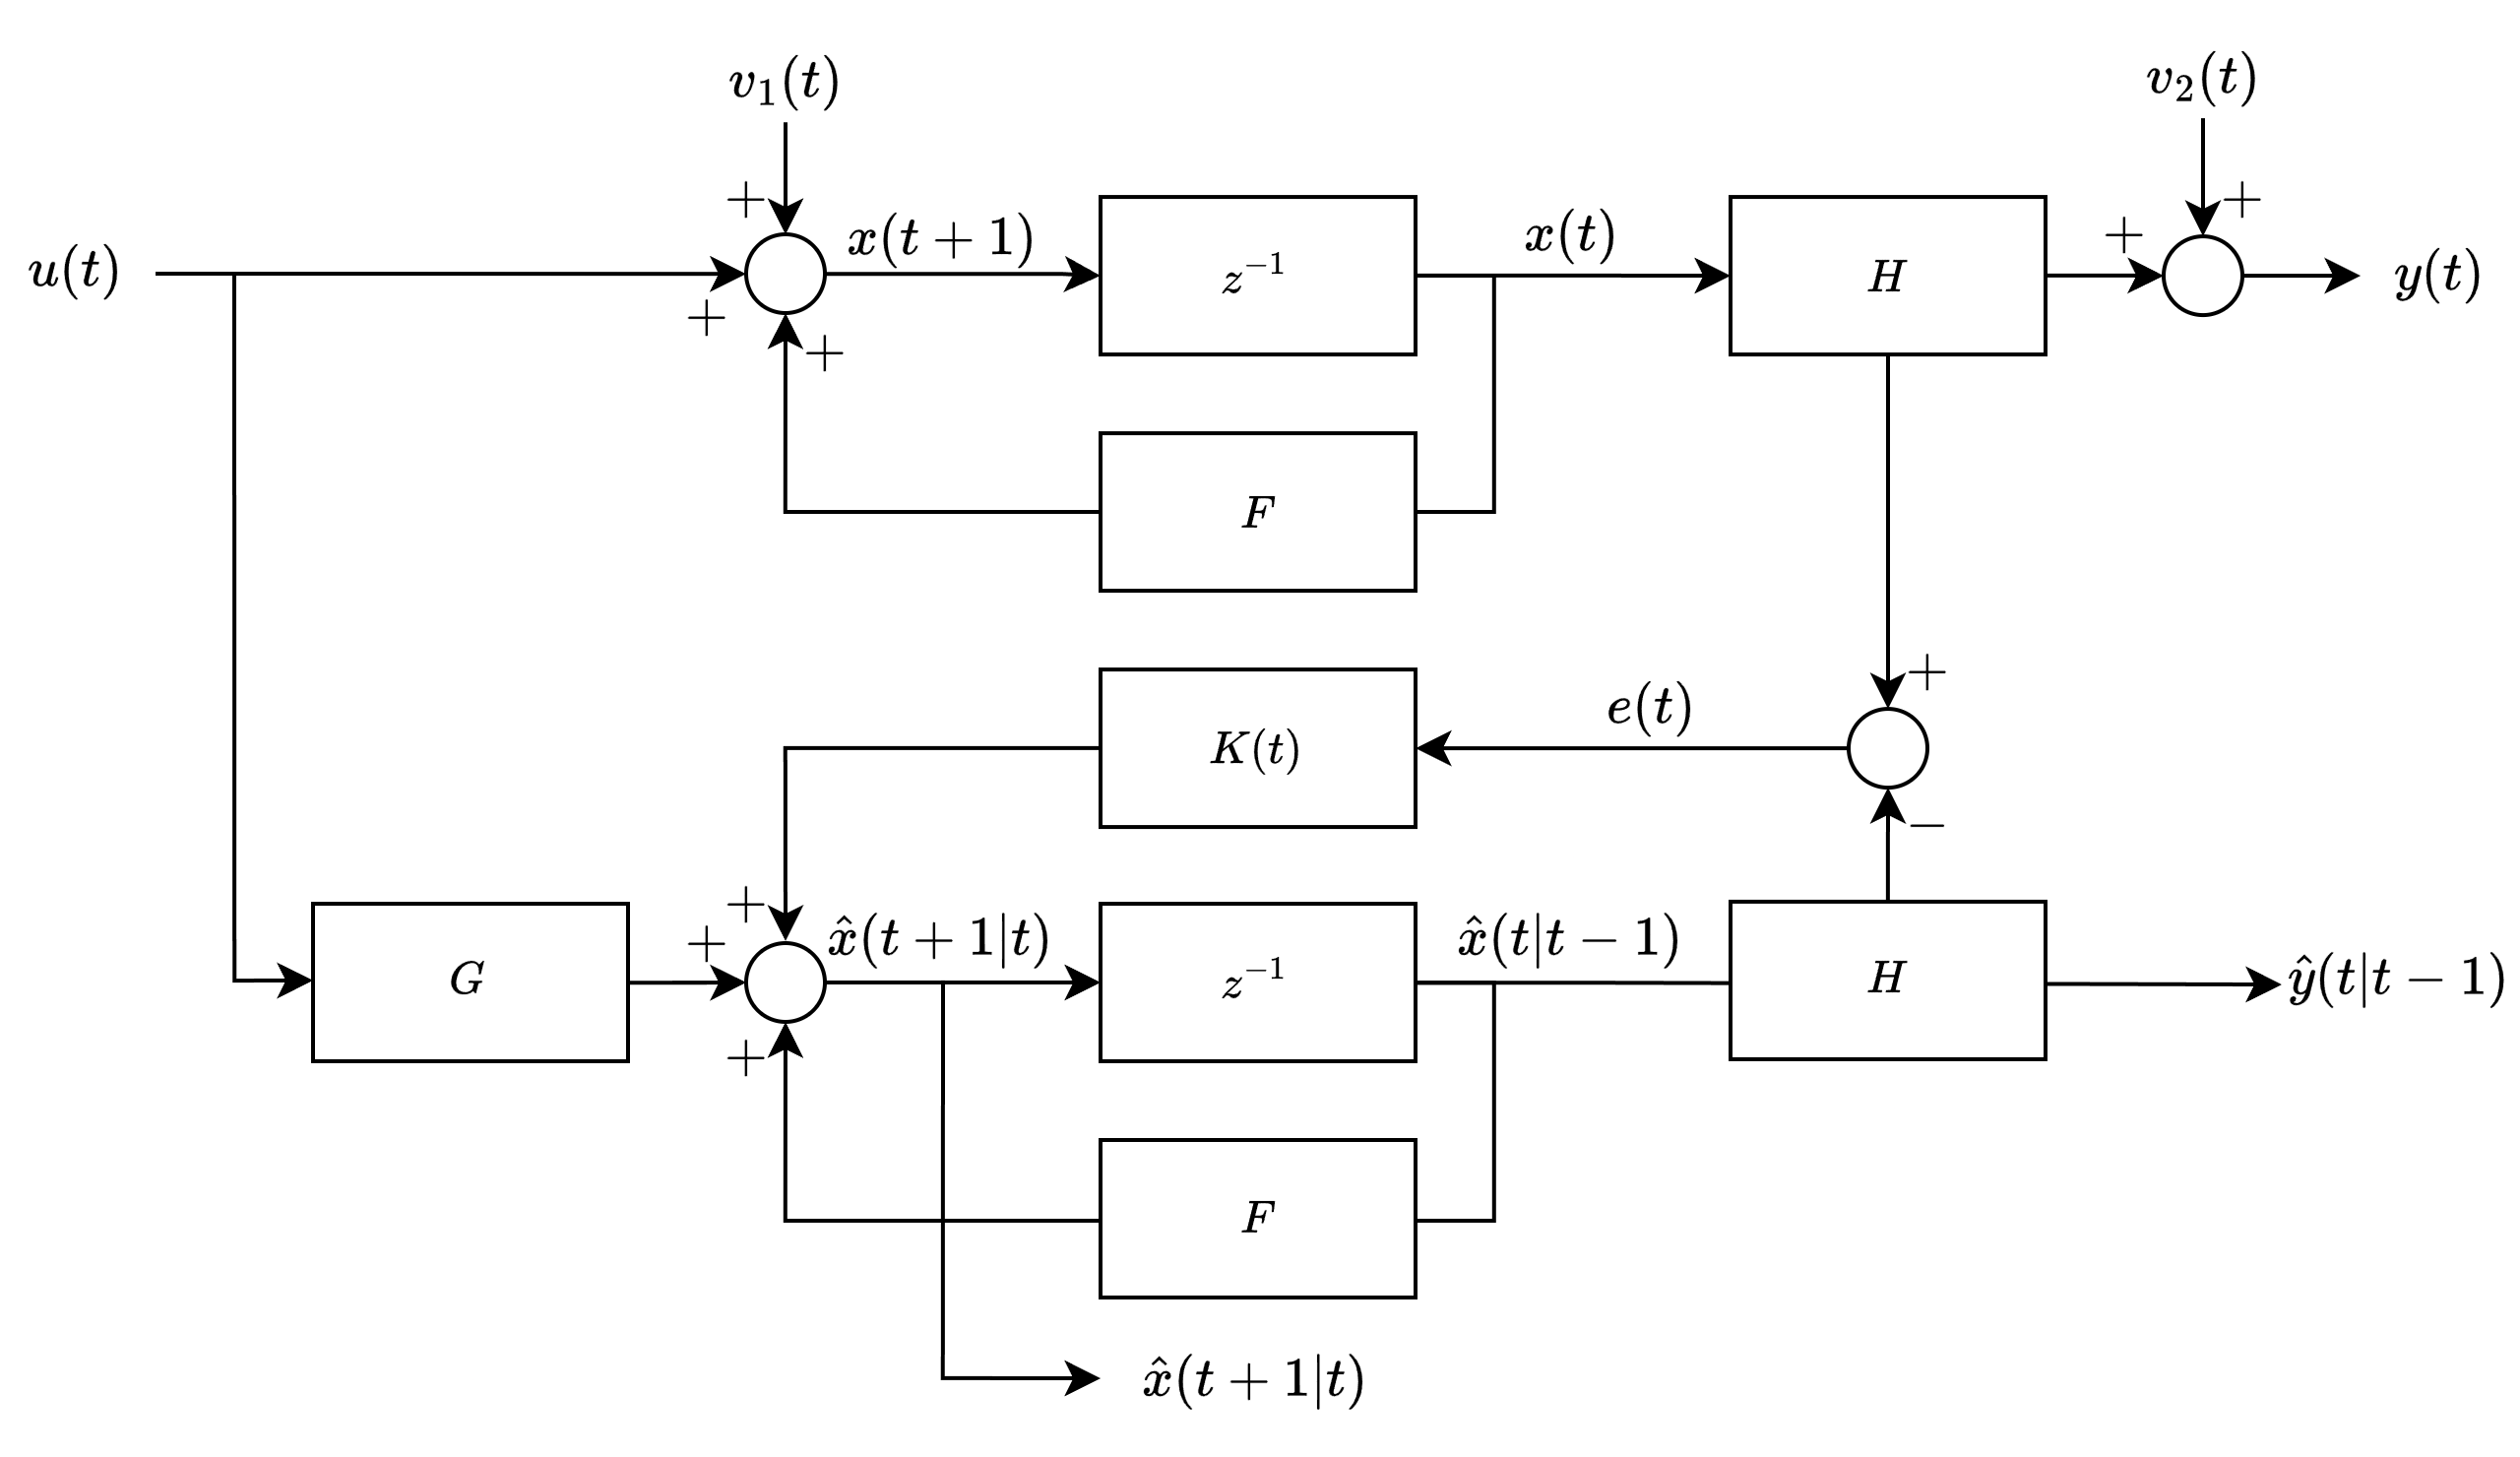
\includegraphics[width=0.75\linewidth]{images/ke.png}
    \caption{Kalman Filtering with eXogenous input}
\end{figure}
Notably, the $K(t)$ and $P(t)$ terms remain unchanged from the formulas without $Gu(t)$. 
This intuitively makes sense because $Gu(t)$ does not introduce additional uncertainty into the system; rather, it represents a deterministic component added to the system. 
Consequently, the state prediction error $P(t)$ remains unaffected.

\subsection{Time-variant systems}
Consider a system represented by the following equations, where all matrices are time dependent:
\[\begin{cases}
    x(t+1)=F(t)x(t)+G(t)u(t)+v_1(t) \\
    y(t)=H(t)x(t)+v_2(t)
\end{cases}\]
In this scenario, even with time-variance in the system matrices, the Kalman Filter equations remain identical to those of time-invariant systems.